\chapter{Multirate implementation}
The chapter will describe the three functions which is used in the multirate stages.
\begin{itemize}
\item void downFunc1(int16 dataIn);
\item int16 delayB1(int16 dataIn);
\item int16 upFunc1(int16 dataIn,int16 band);
\end{itemize}
Where downFunc1 is used to decimate and spectral subtract the input sample, delayB1 is used to delay a sample by x samples and upFunc1 is used interpolate the input sample (dataIn) and add the input sample (band) to the interpolated signal. In both downFunc1 and upFunc1 a filter function is used called FIR1 which runs a FIR filter on a data array, which also will be decribed in this chapter. 


\section{Decimation and spectral subtraction implementation}
The decimation block is described in \textbf{XX} and is seen on \autoref{fig:DownsamplingSimulationCopy}.
\begin{figure}[H]
    \centering
	\includegraphics[width=0.7\textwidth, page=2]{Simulation}
    \caption{Decimation block diagram}
    \label{fig:DownsamplingSimulationCopy}
\end{figure}
The block contains different components which has to be implemented:
\begin{itemize}
\item Reading data in.
\item FIR filtering.
\item Spectral subtraction.
\item Downsampling and outputting. 
\end{itemize}
An input sample must be read into a buffer of the size equal to the filter taps. The decimation filter has 51 taps and is described in \autoref{sec:decFilter}, so the buffer must be of equal size, but the buffer can be designed in a number of ways:
\begin{itemize}
\item First in first out (FIFO).
\item Circular
\end{itemize} 
A FIFO buffer is the simple of the two buffer types but it also requires more computation power than a circular buffer. This is because in a FIFO buffer all data must be moved as seen in \autoref{fig:FIFO} while in a circular buffer, see \autoref{fig:Circular}, a pointer can be moved so instead of moving data the pointer moves to the oldest data. So instead of costing the same number of instructions equal to size of the buffer, it only cost the setup of the circular buffer and one instruction per move.   
\begin{figure}[H]
\centering
\begin{subfigure}[t]{0.49\textwidth}
    \centering
	\includegraphics[width=0.6\textwidth]{FIFO.png}
	\caption{FIFO buffer.}
	\label{fig:FIFO}
\end{subfigure}
\begin{subfigure}[t]{0.49\textwidth}
    \centering
	\includegraphics[width=0.4\textwidth]{Circular.png}
	\caption{Circular buffer.}
	\label{fig:Circular}
\end{subfigure}
\caption{Buffer types.}
\label{fig:bufTypes}
\end{figure}
It is choosen to implement a circular buffer because of its cost effectiveness and the implementation is seen on \autoref{ls:ReadingInData}.
\begin{lstlisting}[language={[x86masm]Assembler}, caption = {Reading data in},label={ls:ReadingInData}]
	MOV #0, AC0					; Clear AC0
	OR #dataIn1,AC0				; Load address of input data into AC0
	ADD *(#i1),AC0				; Add the addr with the value of the data pointer (Point to oldest data)
	MOV AC0,XAR0				; Move the addr to AR0
	MOV T0, *AR0				; Move the value in T0 to the address
	ADD #1,*(#i1)				; Increment the data pointer
	ADD #1,*(#d1)				; Increment the delay pointer
	CMP *(#i1)==#51,TC1			; Check if the data pointer should reset to 0
	CALLCC resetPtri1, TC1
	CMP *(#d1)==#51,TC1			; Check if the delay pointer should reset to 0
	CALLCC resetPtrd1, TC1
\end{lstlisting}
Where: \\
- dataIn1, is the pointer which points to the start adress of the buffer. \\
- i1, is a pointer which points to the oldest data in the buffer. \\
- d1, is a pointer which is delayed 25 (filter delay) in relation to i1. 

The start adress of the buffer "dataIn1" is added with the oldest sample number in the buffer "i1", which gives the adress of the oldest data. The new sample is moved over in "T0" and overwrites the oldest data in the buffer. The pointers are incremented and if the equal to the size of the buffer they are reset to 0 using calls to resetPtri1 and resetPtrd1.

When data is read the FIR routine is called which runs the FIR filter on the data, this is implemented as seen on \autoref{fig:FirImp}.
\begin{figure}[H]
\centering
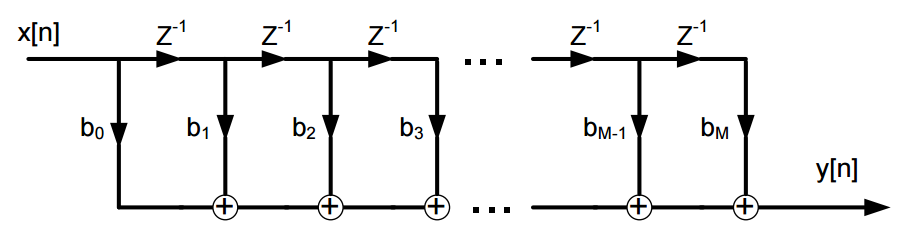
\includegraphics[width=0.9\textwidth]{FIRImp.png}
\caption{FIR implementation.}
\label{fig:FirImp}
\end{figure}

Every tap is a coefficient and a sample multiplied and all taps are accumulated which gives the output of the filter. This is done with the multiply accumulate (MAC) instruction, as seen in \autoref{ls:FIRimp}.
\begin{lstlisting}[language={[x86masm]Assembler}, caption = {FIR algorithm.},label={ls:FIRimp}]
	MOV #0, AC1					; Clear AC1
	MOV #51, BK03				; Set buffer size to filter order
	MOV #0, AC0
	OR #dataIn1,AC0				; Load AC0 with the data start addr
	MOV AC0,XAR2				; AR2 as coefficient pointer
	MOV mmap(AR2),BSA23        	; Set up base address for AR2
	MOV *(#i1),AC0				; Start the circular buffer at i'th data
	MOV AC0,AR2					; Start from the i'th data
	bset AR2LC					; Set pointer as circular
	MOV #bCoeff,AC0				; Load AC0 with the addr of the coefficients
	MOV AC0, AR1				; Load AR0 with the val of AC0
	RPT #50						
	MAC *AR2+,*AR1+,AC1 		; Do filter convolution
	SFTL AC1, #-15				; Bit shift to fit Q15
	MOV AC1,T0     				
	RET
\end{lstlisting}
Where: \\
- bCoeff, is a pointer to the start of the coefficients in memory. 

Data is first moved into one of the five internal circular buffers with line (1-8). The internal circular buffers uses specific registers as buffers and pointers, but when the pointer is incremented at the end of the buffer it automatically returns to the start without the need of a reset function. When the circular buffer is set up for the data, the adress of the coefficients are moved into the "AR1", hereby both data and coefficients pointers can be incremented without error for the number of repeats (51) nescessary to calculate the output of the filter. 

The output is calculated as mentioned before with the MAC instruction which is repeated 51 times while the pointers are incremented every time a MAC is performed. When all taps are acumulated the result is shiftet 15 times with the barrel shifter because a multiplication results in a 32-bit result with two sign bits, where the 15 most significant value bits are taken as the output of the filter.

Spectral subtraction is done by using the output of the FIR routine "T0" and a delayed input sample pointed to by "d1" as seen in \autoref{ls:specSub} which gives the first output "band1".

\begin{lstlisting}[language={[x86masm]Assembler}, caption = {Spectral subtraction.},label={ls:specSub}]
	MOV #0, AC0
	OR #dataIn1, AC0			
	ADD *(#d1), AC0				
	MOV AC0, AR0
	MOV *AR0,AC0
	SUB T0, AC0
	MOV AC0,*(#band1)
\end{lstlisting}

The last function of decimation block is downsampling the output of the FIR routine. This is done by not overwriting the output every second time which is done with a counter as seen on \autoref{ls:downsampling}.

\begin{lstlisting}[language={[x86masm]Assembler}, caption = {Downsampling.},label={ls:downsampling}]
	CMP *(#k1)==#0, TC1
	CALLCC DownOut1, TC1
	ADD #1, *(#k1)
	CMP *(#k1)==#2, TC1
	CALLCC resetK1, TC1
\end{lstlisting}
where: \\
- k1, is a counter.

When DownOut1 is called, when "k1" equals 0, a new output is given in "down1" which holds the downsampled output. If "k1" is not 0 a new output is not given, and when "k1" equals 2 it resets. The reason then for running the FIR routine every sample is because of the spectral subtraction which requires a new output every sample. This concludes the implementation of the decimation block which leads to the interpolation block.

\section{delay implemetation}
The delay block delays a sample x times which is done by implementing a circular buffer with a pointer. The input bandx which is one of the outputs from the decimation block is read into a buffer which is the size of the delay the same way as data is read into the decimation buffer as seen on \autoref{ls:delay}.  

\begin{lstlisting}[language={[x86masm]Assembler}, caption = {Delay algorithm.},label={ls:delay}]
	MOV #0, AC0
	OR #delayB1Ptr,AC0			; Load address of input data into AC0
	ADD *(#iD1),AC0				; Add the addr with the value of the data pointer (Point to the oldest data)
	MOV AC0,AR0					; Move the addr to AR0
	MOV T0,T1
	MOV *AR0,T0	
	MOV T1, *AR0				; Move the value in T0 to the address
	ADD #1,*(#iD1)				; Increment the data pointer
	CMP *(#iD1)==#5308,TC1			; Check if the data pointer should reset to 0
	CALLCC resetPtri1, TC1		
\end{lstlisting}

The pointer "D1" always points to the oldest sample which has been delayed x samples, so before it is overwritten it is moved to "TO" which is the output register of the function. When the sample has been moved the new sample can overwrite and it can thereby be delayed x times before it is outputted again.

\section{Interpolation implementation}
The interpolation block is described in \textbf{XX} and is seen on \autoref{fig:upsamplingSimulationCopy}.
\begin{figure}[H]
    \centering
	\includegraphics[width=0.7\textwidth, page=11]{Simulation}
    \caption{Interpolation block diagram}
    \label{fig:upsamplingSimulationCopy}
\end{figure}
The block contains different component which has to be implemented:
\begin{itemize}
\item Reading in data and upsampling.
\item FIR filtering.
\item Gain by two.
\item Spectral addition.
\end{itemize}
Upsampling is described in detail in \textbf{XX}, but it means zero padding a signal, so if the signal is upsampled by there should be inserted a zero in between every sample which result in an increase of Fs by multiple two. The way a sample is read in is the same as \autoref{ls:ReadingInData} but every second time a zero padding function, seen in \autoref{ls:zero}, is called instead of reading in data.  

\begin{lstlisting}[language={[x86masm]Assembler}, caption = {Downsampling.},label={ls:zero}]
	MOV #0, AC0
	OR #dataInUp1,AC0			; Load address of input data into AC0
	ADD *(#iUp1),AC0			; Add the addr with the value of the data pointer (Point to the oldest data)
	MOV AC0,AR0					; Move the addr to AR0
	MOV #0, *AR0				; Move the value in T0 to the address
	RET
\end{lstlisting}
Which is controlled by a counter in the way as \autoref{ls:downsampling}, with the difference that it reads in data when the counter is 0, reads in a 0 if the counter is 1 and reset if the counter is 2. It should be noted that the data buffer is twice the size of the filter because the order is equal which means the number of taps is odd, which result in an error in memory if the buffer size is odd. This is because if a zero is inserted after every sample, then in an odd buffer size a zero is inserted next to another zero instead next to data when the data pointer is reset, which will not happen in an equal size buffer. 

When data is loaded into the buffer the FIR routine as showed in \autoref{ls:FIRimp} runs with the interpolation filter descirbed in \autoref{sec:IntFilter}, so this will not be described again. 

The output is then multiplied by two because of the zero padding, which is done with the barrel shifter, and lastly the shifted output is added with a band input. This is then the output of the interpolation block.



